% Grafic 1: Victime civile
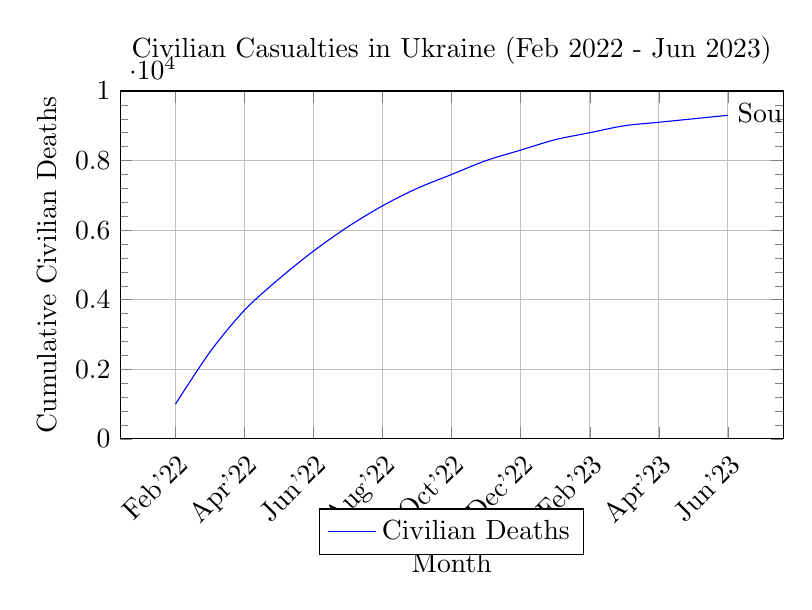
\begin{tikzpicture}
    \begin{axis}[
        title={Civilian Casualties in Ukraine (Feb 2022 - Jun 2023)},
        xlabel={Month},
        ylabel={Cumulative Civilian Deaths},
        grid=major,
        width=10cm,
        height=6cm,
        xtick={1,3,5,7,9,11,13,15,17},
        xticklabels={Feb'22,Apr'22,Jun'22,Aug'22,Oct'22,Dec'22,Feb'23,Apr'23,Jun'23},
        xticklabel style={rotate=45,anchor=north east},
        ymin=0,
        ymax=10000,
        minor y tick num=4,
        legend style={at={(0.5,-0.2)},anchor=north}
    ]
    \addplot[smooth,mark=none,blue] coordinates {
        (1, 1000) (2, 2500) (3, 3700) (4, 4600) (5, 5400) 
        (6, 6100) (7, 6700) (8, 7200) (9, 7600) (10, 8000) 
        (11, 8300) (12, 8600) (13, 8800) (14, 9000) (15, 9100) 
        (16, 9200) (17, 9300)
    };
    \legend{Civilian Deaths}
    \node at (axis cs:17,9300) [anchor=west] {Source: UN OHCHR \cite{un_2023}};
    \end{axis}
\end{tikzpicture}

\vspace{1cm}

% Grafic 2: Refugiați
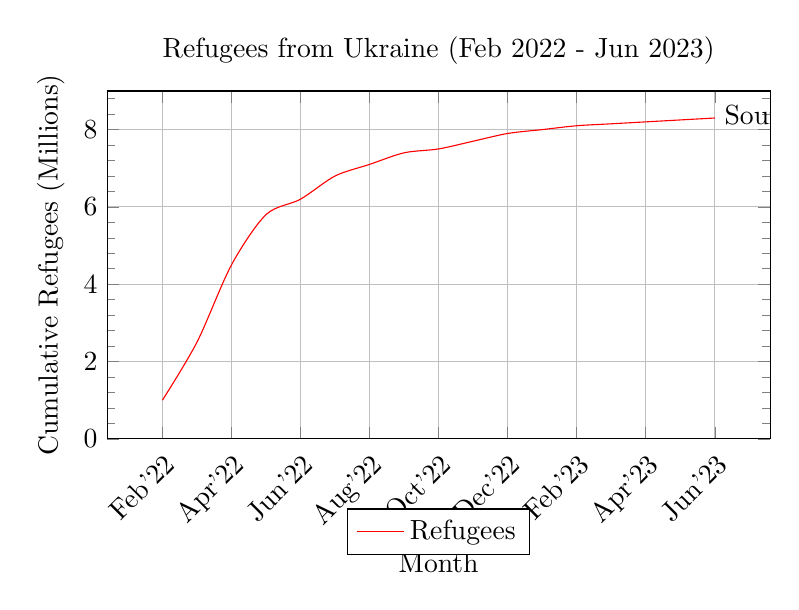
\begin{tikzpicture}
    \begin{axis}[
        title={Refugees from Ukraine (Feb 2022 - Jun 2023)},
        xlabel={Month},
        ylabel={Cumulative Refugees (Millions)},
        grid=major,
        width=10cm,
        height=6cm,
        xtick={1,3,5,7,9,11,13,15,17},
        xticklabels={Feb'22,Apr'22,Jun'22,Aug'22,Oct'22,Dec'22,Feb'23,Apr'23,Jun'23},
        xticklabel style={rotate=45,anchor=north east},
        ymin=0,
        ymax=9,
        minor y tick num=4,
        legend style={at={(0.5,-0.2)},anchor=north}
    ]
    \addplot[smooth,mark=none,red] coordinates {
        (1, 1) (2, 2.5) (3, 4.5) (4, 5.8) (5, 6.2) 
        (6, 6.8) (7, 7.1) (8, 7.4) (9, 7.5) (10, 7.7) 
        (11, 7.9) (12, 8.0) (13, 8.1) (14, 8.15) (15, 8.2) 
        (16, 8.25) (17, 8.3)
    };
    \legend{Refugees}
    \node at (axis cs:17,8.3) [anchor=west] {Source: UNHCR \cite{unhcr_2023}};
    \end{axis}
\end{tikzpicture}
